\section{Análise de Valor}
\label{sec:chap02_valueanalysis}
Até ao momento, deu-se o contexto do trabalho a ser desenvolvido, de forma a perceber a realidade atual dos sistemas de controlo de produção. Contudo, é preciso perceber qual o impacto que a solução a ser desenvolvida terá no produto e no mercado no qual se insere. Visto que o módulo a desenvolver será integrado num produto já existente, analisa-se a oportunidade de negócio que surge com a nova funcionalidade.

\subsection{O Processo de Inovação}
De acordo com~\textcite{ffe_effectivemethods_tools_techniques}, o processo de inovação, representado na Figura~\ref{fig:inovation_process}, está dividido em três áreas -- o \gls{ffe}, \gls{npd} e a comercialização -- que correspondem às fases inerentes ao \gls{ncd}, um modelo desenvolvido por um conjunto de empresas, com o objetivo de \inquotes{[...]~fornecer uma linguagem e compreensão comum para as atividades \textit{front end}}\footnote{Tradução livre de autor. No original \inquotes{[...]~to provide a common language and insights on the front end activities.}.}~\parencite{providing_clarity_common_language_ffe}.

O \gls{ffe} representa uma oportunidade para melhoria de todo o processo de inovação, focando todas as atividades que antecedem o desenvolvimento do produto, com o propósito de potenciar o valor, a importância e a probabilidade de sucesso das fases que se seguem. Ou seja, consiste no investimento do tempo em atividades de discussão da ideia, por forma a identificar e estruturar o problema ou oportunidade~\parencite{ffe_effectivemethods_tools_techniques, ffe_theoretical_model}. Porém, as atividades inerentes ao \gls{ffe} são fundamentalmente diferentes da fase \gls{npd}, pelo que se torna necessária a definição de vocabulário específico, permitindo a geração de conhecimento e clara distinção entre as diferentes fases do processo~\parencite{ffe_effectivemethods_tools_techniques}.

\begin{figure}[!ht]
    \centering
    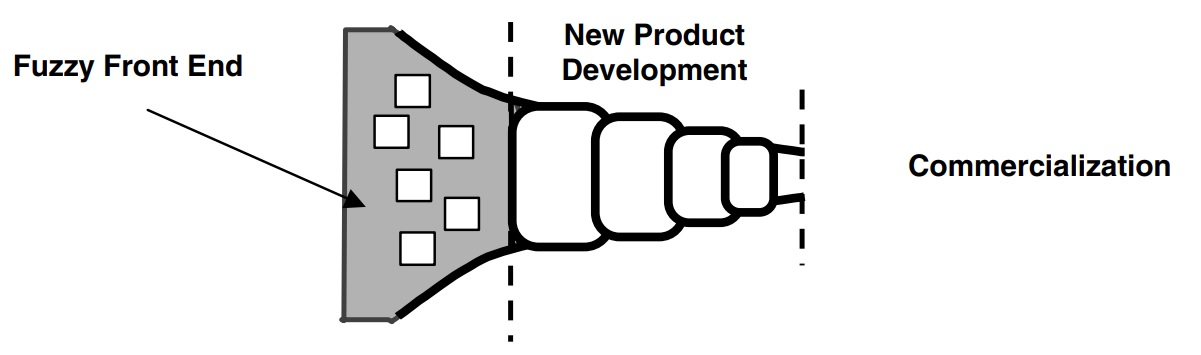
\includegraphics[width=.95\textwidth]{ch02/assets/inovation_process.jpg}
    \caption{O processo de inovação, extraído de~\textcite{ffe_effectivemethods_tools_techniques}}
    \label{fig:inovation_process}
\end{figure}

O modelo \gls{ncd}, demonstrado na Figura~\ref{fig:ncd_model}, baseado num modelo relacional ao invés de um processo linear, visa providenciar uma terminologia para o \gls{ffe}~\parencite{ffe_effectivemethods_tools_techniques}. A área interna define os cinco elementos chave do \textit{Front End of Inovation}: a identificação de oportunidade (\textit{Opportunity Identification}), a análise de oportunidade (\textit{Opportunity Analysis}), a geração e enriquecimento de ideias (\textit{Idea Generation and Enrichment}), a seleção de ideias (\textit{Idea Selection}) e a definição do conceito (\textit{Concept Definition}). O motor central (\textit{Engine}) corresponde à liderança, cultura e estratégia organizacional, que suporta os elementos que compõem o \gls{ffe}, são controláveis pela organização e possibilita a interação entre eles. Já na periferia, encontram-se os fatores de influência (\textit{Influencing Factors}), geralmente incontroláveis pela organização, consistem nas capacidades organizacionais, na estratégia de negócio, no mundo exterior, nomeadamente os canais de distribuição, clientes, fornecedores, concorrentes, política governamental ou legislação, ou quaisquer fatores que possam influenciar todo o processo de inovação~\parencite{ffe_effectivemethods_tools_techniques, providing_clarity_common_language_ffe}.

\begin{figure}[!ht]
    \centering
    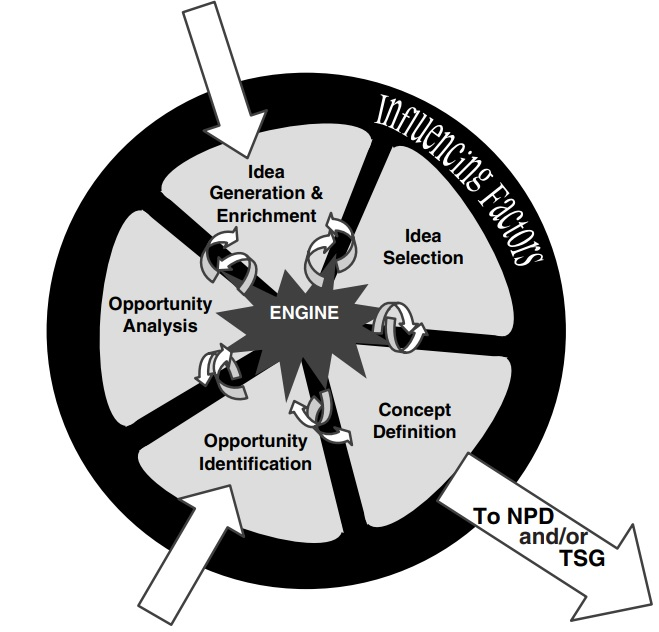
\includegraphics[width=.55\textwidth]{ch02/assets/ncd_model.jpg}
    \caption{A representação do modelo \glsfirst{ncd}, extraído de~\textcite{ffe_effectivemethods_tools_techniques}}
    \label{fig:ncd_model}
\end{figure}

Quanto à representação do modelo, as partes internas são designadas de elementos por oposição a processos, pois estes implicam estrutura, que pode não ser possível ser aplicada. O formato circular indica que é esperado que as ideias fluam, circulem e iterem ao longo dos elementos, por qualquer ordem ou combinação, permitindo o uso dos elementos, repetidamente. Este comportamento é intrínseco às atividades do \gls{ffe}, permitindo uma definição clara do mercado, dos requisitos, dos riscos associados e do plano de negócio, tornando mais eficazes as fases de desenvolvimento e comercialização, devido à redução do tempo total de projeto, fruto da diminuição da repetição de algumas atividades~\parencite{ffe_effectivemethods_tools_techniques}. 

\subsection{O \textit{Fuzzy Front End} de Inovação}
Como mencionado anteriormente, o \gls{ffe} corresponde a um conjunto de atividades geralmente caóticas, imprevisíveis e não estruturadas que antecedem o desenvolvimento de um produto~\parencite{ffe_incremental_platform_breakthrough_products}. Todavia, é preciso perceber a natureza do produto a desenvolver, de forma a melhor enquadrar o processo de inovação.

Segundo~\textcite{ffe_incremental_platform_breakthrough_products}, pode-se caracterizar os produtos de acordo com a extensão da mudança ou do processo: incremental, requer pouca mudança a nível do produto ou do processo, uma vez que geralmente consiste na redução de custos, melhoria, extensão ou reposicionamento no mercado de produtos já existentes; plataforma, estabelecem uma arquitetura básica para uma nova geração de produtos ou processos; pioneiro, envolve uma mudança significativa no processo ou produto.

O presente trabalho visa o desenvolvimento dum módulo de linguagem natural para o {\productname}, uma plataforma já estabelecida, ou seja, trata-se de uma extensão ao produto já existente, enquadrando-se no tipo incremental. A ideia surge do processo de planeamento estratégico da empresa com a finalidade de trazer novas funcionalidades aos seus clientes, melhorando a qualidade do produto. Portanto, nas secções seguintes, aplica-se a metodologia explicitada, no sentido de enriquecer a proposta de projeto apresentada pela {\companyname}.

\subsubsection{Identificação da Oportunidade}
O \gls{pln} é uma área de investigação que explora a forma como os computadores podem manipular a linguagem natural (texto ou voz) para executar determinadas tarefas. Aplica-se em diversos campos de estudo: tradução, processamento de texto, interfaces com o utilizador, reconhecimento de voz, sistemas periciais~\parencite{nlp}.

\textcite{end_to_end_neural_nli_databases} menciona que, apesar da expressividade da \gls{sql}, os utilizadores necessitam de algum conhecimento técnico para perceber como extrair informação de um sistema, o que conduziu à investigação para o desenvolvimento de interfaces alternativas que permitam aos utilizadores, sem conhecimento técnico, explorar e interagir com os dados, de forma conveniente. Também \textcite{towards_theory_nli_databases} menciona que a necessidade de interfaces de linguagem natural se torna mais evidente, devido ao número de pessoas sem conhecimentos técnicos que acedem a informação através de \textit{browsers} ou telemóveis, tornando paradigmas como o reconhecimento de voz mais atrativos.

Nesse sentido, a {\companyname} tenciona o desenvolvimento do módulo de linguagem natural para que os utilizadores do produto, sem conhecimento orientado às tecnologias de informação, possam fácil, rápida e intuitivamente consultar o sistema. Desta forma, a funcionalidade destaca o produto pelo uso de novas tecnologias, facilita-se a interação com o sistema, reduzindo-se o tempo de formação técnica associado ao mesmo. 

\subsubsection{Análise da Oportunidade}
A pesquisa realizada por~\textcite{roadmap_nlp_research_is}, apresentada na Figura~\ref{fig:number_articles_per_year_nlp}, cuja metodologia consistiu na pesquisa de termos como \inquotes{Natural Language Processing} e \inquotes{NLP} em bases de dados académicas, determina que tem havido uma tendência crescente de interesse por esta área. Nos últimos anos, a quantidade de dados textuais disponíveis nas redes sociais ou em sistemas de comunicação, juntamente com a necessidade de acesso a informação, contribuíram para o avanço e adoção comercial do \gls{pln}~\parencite{roadmap_nlp_research_is}.

\begin{figure}[!ht]
    \centering
    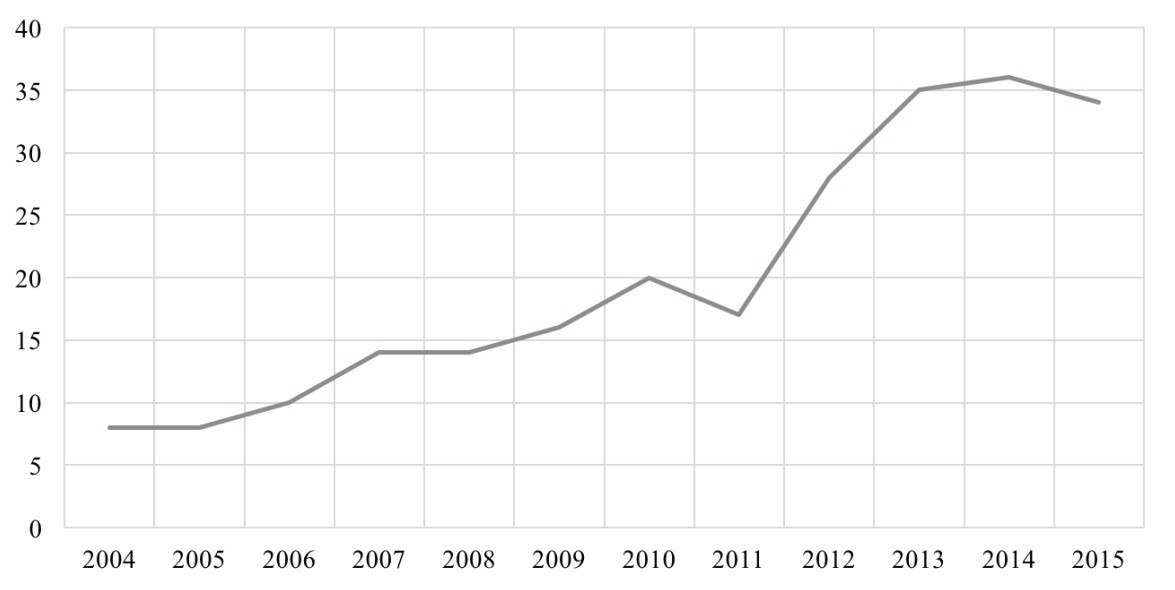
\includegraphics[width=.9\textwidth]{ch02/assets/number_articles_nlp.jpg}
    \caption{Número de artigos de \glsfirst{pln} pesquisados por ano, extraído de~\textcite{roadmap_nlp_research_is}}
    \label{fig:number_articles_per_year_nlp}
\end{figure}

Quanto ao segmento de mercado no qual se integra, cresce a visão de fábricas inteligentes, associadas à quarta revolução industrial, prezando a integração do operador humano num ambiente complexo e rico em dados~\parencite{social_factory}. \textcite{industry40_revolution_future_mes} afirma que a revolução supracitada é já conhecida pelas empresas, o que lhe permite tomar ações no sentido de definir o seu modelo de fabrico e o seu plano de transformação, particularmente na adaptação do \gls{mes} de forma a manter o desempenho, qualidade e agilidade nas desafios espoletados pelas empresas de manufatura. Portanto, a interação entre o ser humano e o sistema pode melhorar o processo de fabrico e potenciar o negócio, na medida em que o operador, em vez do trabalho manual repetitivo que pode facilmente ser automatizado, passa a tomar decisões no processo para resolução de problemas, as quais requerem acesso à informação correta e de forma atempada~\parencite{social_factory}. É nesse sentido que o {\productname} ganha vantagem com o desenvolvimento desta nova funcionalidade.

\subsubsection{Geração, Enriquecimento e Seleção de Ideias}
No seguimento deste assunto, foram realizadas duas reuniões com o supervisor do projeto na {\companyname}, em que foram discutidos alguns requisitos operacionais e de usabilidade, restrições ao desenvolvimento da solução, como a preferência por uso de ferramentas de \gls{pln} que possam ser mantidas internamente e a sua facilidade de utilização, e ideias para futuras implementações, as quais podem ter um impacto na especificação arquitetural do protótipo.

\begin{figure}
    \centering
    \resizebox{\textwidth}{!}{\begin{tikzpicture}
  \path[mindmap, concept color=black!50,text=white,
    every node/.append style={concept, minimum size=0.5cm, inner sep=0.2mm},
    level 1 concept/.append style={text width=1.5cm,font=\scriptsize},
    level 2 concept/.append style={text width=1.27cm,font=\tiny\bfseries,level distance=50}
  ]
    % Root
    node[text width=2.3cm,font=\small] {Projeto}
    %
    [clockwise from=0]
    child[concept color=black!25,text=black,level distance=80] { node {Restrições}
      [clockwise from=120]
      child { node {Uso Interno} }
      child { node {Custo} }
      child { node {Eficiência} }
      child { node {Aprendizagem da Ferramenta} }
      child { node {Usabilidade da Solução} }
    }
    %
    child[concept color=black!25,text=black,level distance=115] { node {Requisitos}
      [clockwise from=0]
      child { node {Semântica Temporal} }
      child { node {Semântica de Domínio} }
      child { node {Integração com Produto} }
      child { node {Auto-aprendizagem} }
    }
    %
    child[concept color=black!25,text=black,level distance=90] { node {Estado da arte} 
      [clockwise from=-115]
      child { node {Soluções Análogas} }
      child { node {Ferramentas} }
    }
    %
    child[concept color=black!25,text=black,level distance=75] { node {Tecnologia}
      [counterclockwise from=75]
      child { node {PLN} }
      child { node {Interfaces de Linguagem Natural} }
      child { node {\textit{Data Warehouses}} }
    }
    %
    child[concept color=black!25,text=black,level distance=125] { node {Clientes}
      [counterclockwise from=-30]
      child { node {Semi\\condutores} }
      child { node {Equipamentos Médicos} }
      child { node {Montagem Eletrónica} }
      child { node {Energia Solar} }
      child { node {Outros} }
    }
    child[concept color=black!25,text=black,level distance=135] { node {Utilizadores}
      [counterclockwise from=-35]
      child { node {Engenheiros de Produção} }
      child { node {Engenheiros de Qualidade} }
      child { node {Responsáveis de Linha} }
      child { node {Operadores} }
    };
\end{tikzpicture}}
    \caption{\textit{Mindmap} das ideias e conceitos gerados}
    \label{fig:mindmap}
\end{figure}

Em relação às ideias e conceitos contempladas no \textit{mindmap} da Figura~\ref{fig:mindmap}, o presente projeto pretende dar resposta a praticamente todos, tendo em consideração que, numa fase inicial, o cumprimento de todos é praticamente inatingível. A descrição de cada conceito é feito de seguida:

\begin{itemize}
    \item
    {
        \textit{Tecnologia} -- a ideia inerente ao trabalho assenta sobre as temáticas de \gls{pln}, especificamente Interfaces de Linguagem Natural, e \textit{Data Warehouses}. Esta consiste no estudo aprofundado deste tipo de interfaces orientado à consulta em armazéns de dados e disseminação do conhecimento internamente, para que no futuro, o projeto possa ter continuidade;
    }
    \item
    {
        \textit{Estado da Arte} -- abordagem de ferramentas e soluções análogas, com o objetivo de especificar uma arquitetura para o sistema. Este processo dá origem aos documentos de especificação que devem ser usados para consulta por parte dos desenvolvedores, quer numa perspetiva de conhecimento arquitetural, quer das ferramentas que são usadas;
    }
    \item
    {
        \textit{Clientes} -- uma vez que a {\companyname} possui clientes com diferentes realidades, a ideia é que o módulo final esteja preparado para elaborar consultas em qualquer domínio, de forma configurada ou cerne da solução. Contudo, como já abordado anteriormente, no contexto deste trabalho, apenas um domínio será considerado;
    }
    \item
    {
        \textit{Utilizadores} -- a solução deverá responder às necessidades de qualquer utilizador, desde os mais técnicos (Engenheiros de Produção) aos menos técnicos (Operadores). Porém, o protótipo terá em consideração os utilizadores mais comuns do {\productname};
    }
    \item
    {
        \textit{Restrições} -- nesta temática, foram discutidas alternativas de como avaliar o custo de uma ferramenta proprietária, uso de ferramentas \textit{Open Source} ou o desenvolvimento interno da própria biblioteca de \gls{pln}, para garantir que não existem dependências externas à plataforma, a eficiência da solução em contexto produtivo, a facilidade de aprendizagem e usabilidade da mesma. Assim, a usabilidade da solução será estudada a partir do mecanismo de \textit{feedback} provido no módulo e através de inquéritos aos utilizadores, o que também se aplica para a aprendizagem da ferramenta. Relativamente aos restantes tópicos, não houve conclusão acerca das ideias a serem selecionadas;
    }
    \item
    {
        \textit{Requisitos} -- pressupõe-se o uso de auto-aprendizagem para adaptação automática do módulo ao \textit{feedback} do utilizador, ainda que para o protótipo, a resposta a uma simples pergunta como \inquotes{A resposta obtida foi-lhe útil?} é suficiente. Também a integração com o produto, quer a nível aplicacional, quer a nível de processo deve ser considerada, o que resultará na organização de \textit{meetups} com as equipas responsáveis pelo processo de manutenção da plataforma. Quanto aos restantes conceitos, não houve conclusão acerca das ideias selecionadas.
    }
\end{itemize}

\subsubsection{Definição do Conceito}
Todo o processo presente no modelo \gls{ncd} de \gls{ffe} culmina com a definição do conceito, a fase que encaminha o projeto para a implementação~\parencite{ffe_effectivemethods_tools_techniques}.

O presente trabalho, denominado de \inquotes{Natural Language Querying} consiste no desenvolvimento de um módulo de linguagem natural para interface com o {\productname}. Este módulo permitirá a consulta e pesquisa de estados do processo de fabrico por utilizadores com pouco ou nenhum conhecimento associado a tecnologias de informação, garantindo a interação com o sistema de uma forma simples, fácil e intuitiva, melhorando o processo numa perspetiva de apoio à decisão (ver Secção~\ref{sec:chap01_problem}). Os objetivos deste projeto estão descritos na Secção~\ref{sec:chap01_objectives}, a metodologia e critérios de sucesso na Secção~\ref{sec:chap01_solutionevaluation}, e o respetivo plano de trabalho no Capítulo~\ref{sec:chap01_workmethodology}.

O projeto traz benefícios para a empresa e o seu produto, pela adoção de tecnologia de \gls{pln} num contexto industrial, pela melhoria de usabilidade do sistema e pela evolução no processo de apoio à decisão dos seus clientes. Uma vez que o {\productname} é um produto bem posicionado no mercado, não se esperam riscos a nível comercial. Contudo, a uso de tecnologia recente, cujos conceitos não estão totalmente estudados e cujos trabalhos de investigação são limitados, pode provocar atrasos no desenvolvimento do projeto ou incumprimento do orçamento definido. Não obstante, o projeto avança com o desenvolvimento de um protótipo, fase que decidirá a inclusão do módulo na plataforma da {\companyname}.
